\documentclass{article}

\usepackage{fancyhdr}
\usepackage{hyperref}
\usepackage{dirtree}
\usepackage{geometry}
\usepackage{graphicx}
\usepackage{subcaption}



\hypersetup{
    colorlinks=true,
    linkcolor=blue,
    urlcolor=blue,
}

\title{Angry Birds Game in Python \\ with PYGAME}
\author{Sagar V \\ CS-104 Project}
\date{Spring 2024--25}

\pagestyle{fancy}
\lhead{PYGAME - ANGRY BIRDS}
\rhead{Sagar V}

\begin{document}
\maketitle

\begin{abstract}
    This report is a summary of the development process of me making the Angry Birds Game in Python using PYGAME.
    It consists of the game's concepts, design, implementation, and the challenges encountered during development.
    The report seeks to offer a detailed overview that allows for understanding and playing the game without needing direct access to its source code.
\end{abstract}

\tableofcontents
\newpage

\section{Introduction}\label{sec:introduction}
This is a 2 player Angry Birds game where the goal is to destroy the opponent's fortress before your own is destroyed.
You achieve this by using multiple birds of your choice and one special ability.
It also consists of unique themes to add to the battle.
Whoever destroys the other persons fortress \emph{first}, \textbf{wins}.

\section{Modules}\label{sec:modules}
The external modules used are:
\begin{itemize}
    \item \texttt{pygame-ce} - This is the basis of the entire game. It is the more frequently updated community version of the package pygame.
    \item \texttt{sys} - This is the package through which we control system actions, like closing the game window.
    \item \texttt{time} - This package provides various time related functions such as \texttt{time.sleep()} which pauses the execution for the given time
    \item \texttt{random} - This package is used to generate various sets of random numbers.
    \item \texttt{numpy} - This package is used to handle arrays. We use it particularly to store the block objects in an array
    \item \texttt{math} - This package provides various mathematical funtions like \texttt{math.sin()} or \texttt{math.cos()}
    
\end{itemize}

\section{Directory Structure}\label{sec:dir}
The project directory is as follows:

\dirtree{%
    .1 Angry\_Birds/.
    .2 Modules/.
    .3 loading\_screen.py.
    .3 Main\_Menu.py.
    .3 player\_names.py.
    .3 theme\_select.py.
    .3 bird\_select.py.
    .3 play.py.
    .3 winner.py.
    .3 birds.py.
    .3 blocks.py.
    .3 players.py.
    .3 settings.py.
    .2 Media/.
    .2 main.py.
}

\begin{itemize}
    \item \textbf{main.py} -- The main game loop
    \item \textbf{Media} -- Contains the audio, image and font files
    \item \textbf{Modules} -- Contains the core modules of the game 
    \begin{itemize}
        \item \textbf{loading\_screen.py} -- The module which contains and displays loading screen images and objects 
        \item \textbf{Main\_Menu.py} -- The module which contains and displays main menu images and objects
        \item \textbf{player\_names.py} -- The module which displays the interface to enter the player names
        \item \textbf{theme\_select.py} -- The module which displays the interface to select the theme of the game
        \item \textbf{bird\_select.py} -- The module which displays and computes the interface to select birds of each player
        \item \textbf{play.py} -- The main game running module which displays the game. Contains the core mechanics of the game
        \item \textbf{winner.py} -- Displays the winner of the game
        \item \textbf{birds.py} -- Contains the \texttt{Bird} class which handles the bird objects in the game
        \item \textbf{blocks.py} -- contains the \texttt{Blocks} class which handles the block objects in the game
        \item \textbf{players.py} -- Contains the \texttt{Players} class which contains all the attributes of the player like name, score etc.
        \item \textbf{settings.py} -- Contains the constants and global variables used throughout the program
    \end{itemize}
    
\end{itemize}

\section{Running the Game}\label{sec:running}
\subsection{Prerequisites}\label{subsec:prereq}
Requires \texttt{python} already installed. If not installed, refer \href{https://www.python.org/downloads/}{Python download.}\\
Also requires \texttt{pygame-ce} or \texttt{pygame} package. If not installed, refer \href{https://www.pygame.org/wiki/GettingStarted}{\texttt{pygame} docs} or \href{https://pypi.org/project/pygame-ce/}{\texttt{pygame-ce} docs.}\\
After ensuring that both are installed, the game can by run by simply running any of the two:\\ \\
\texttt{python3 main.py}\\ \\
\texttt{python main.py}

\subsection{Rules}
\begin{itemize}
    \item Press \textbf{ENTER} after entering each Player's name for it to be registered into the system.
    \item Each player can choose \textbf{upto 3 birds} of their choice. They receive any of those 3 birds by a \textbf{random algorithm} which cycles through them.
    \item Different birds do different damages to different blocks:
    \begin{itemize}
        \item Red does \textbf{20 damage} to all Blocks
        \item Chuck does \textbf{30 damage} to \textbf{Wood} but \textbf{15 damage} to other blocks
        \item Bomb does \textbf{30 damage} to \textbf{Stone} but \textbf{15 damage} to other blocks
        \item Blue does \textbf{30 damage} to \textbf{Ice} but \textbf{15 damage} to other blocks
        \item Stella does \textbf{40 damage} to \textbf{Block of your choice} but \textbf{10 damage} to other blocks
    \end{itemize}
    \item If a bird goes out of bounds or slows down a lot, it does no damage.
    \item Each block has 60 health. A block disappears when there is \textbf{$ \geq 60$ damage} done to it
    \item The blocks are also randomly generated. They are the same for both players to keep it fair.
    \item Each player gets a \textbf{single use} of special ability, \textbf{Mighty Eagle} in the game. Right click during bird flight before collision to activate the ability. The special ability instanty annihilates any block in its path.
    \item The person who destroys the blocks first wins. If Player 1 destroys it first, however, Player 2 gets another chance to keep it fair.
\end{itemize}


\subsection{Gameplay}\label{subsec:gameplay}
Here we explore how it really is to play the game. The following order of subsections is the actual order of gameplay.\\ There are \textbf{back buttons} everywhere and \textbf{quit buttons} in some screens to enable smooth navigation:

\subsubsection{Loading Screen}
The game begins with a loading screen with a dynamically moving loading bar[\ref{fig:Load}]
\begin{figure}[h]
    \centering
    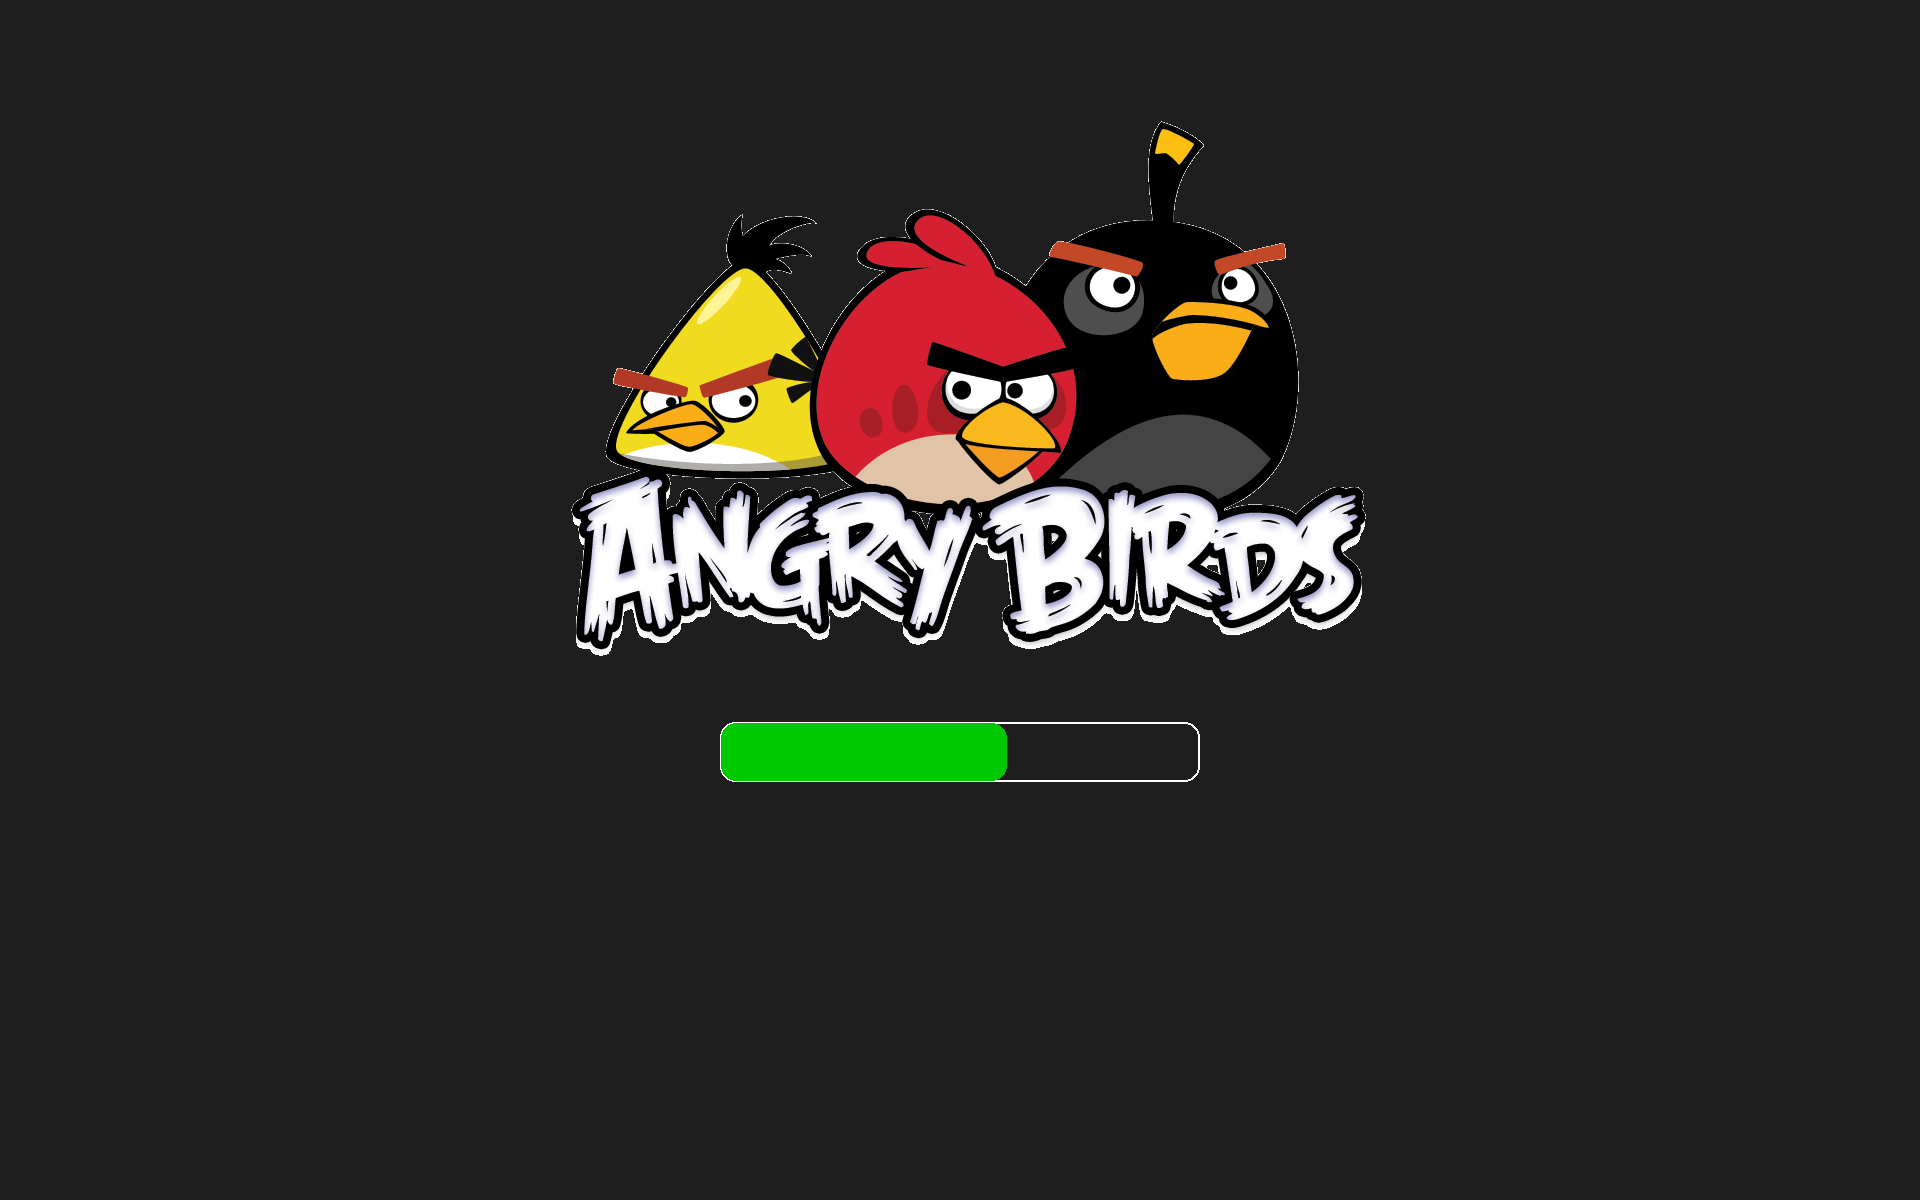
\includegraphics[width=0.5\textwidth]{Loading.png}
    \caption{Loading Screen}\label{fig:Load}
\end{figure}
\newpage
\subsubsection{Main Menu}
This is the main menu from which we choose to either \textbf{PLAY} or \textbf{QUIT}[\ref{fig:Menu}]\\There is also a mute/unmute button for easy volume control.
\\There is also intro music which plays as soon as we enter this screen.
\begin{figure}[h]
    \centering
    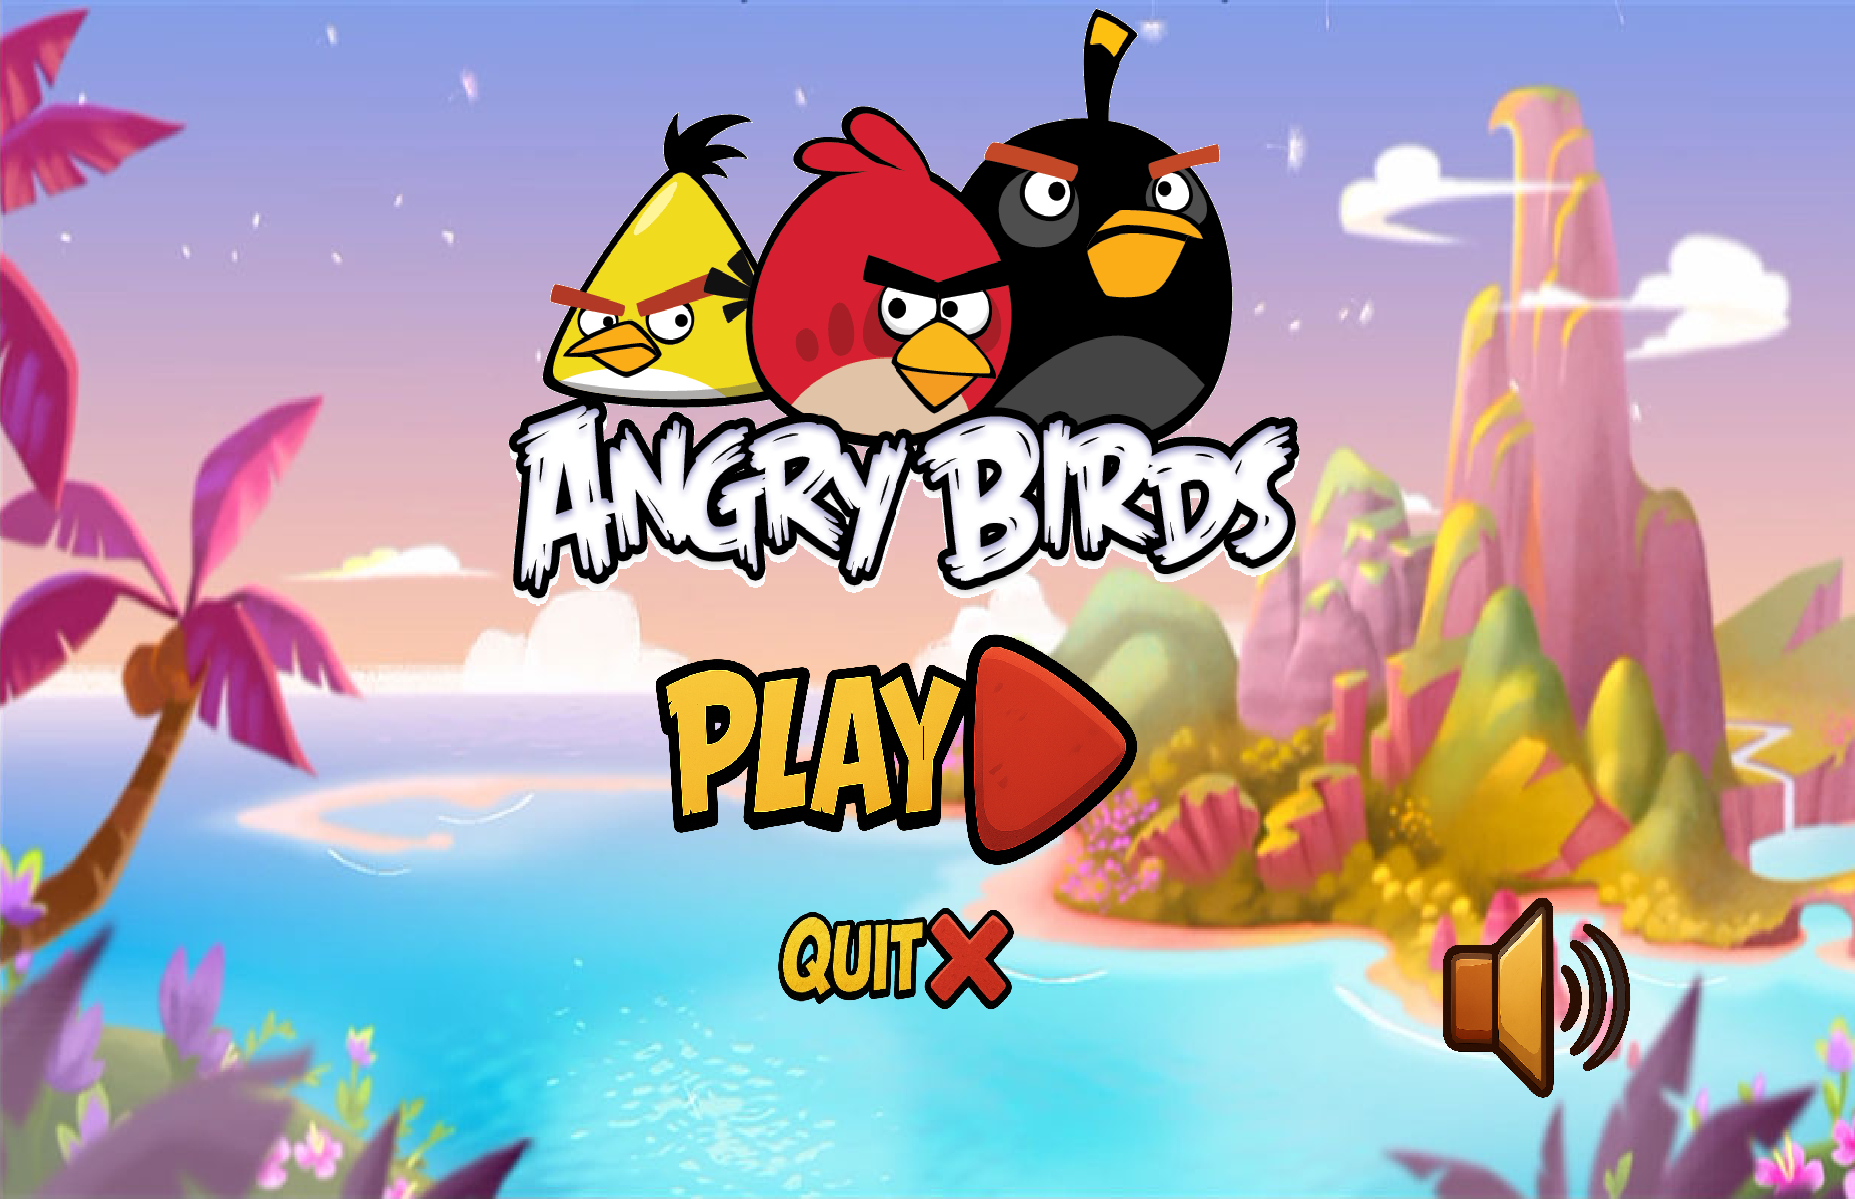
\includegraphics[width=0.5\textwidth]{Menu.png}
    \caption{Main Menu}\label{fig:Menu}
\end{figure}

\subsubsection{Player Naming}
This is where we enter the names of the Players[\ref{fig:Name}]. The selected box is highlighted by the corresponding player colours:\\Yellow for Player 1\\Red for Player 2
\begin{figure}[h]
    \centering
    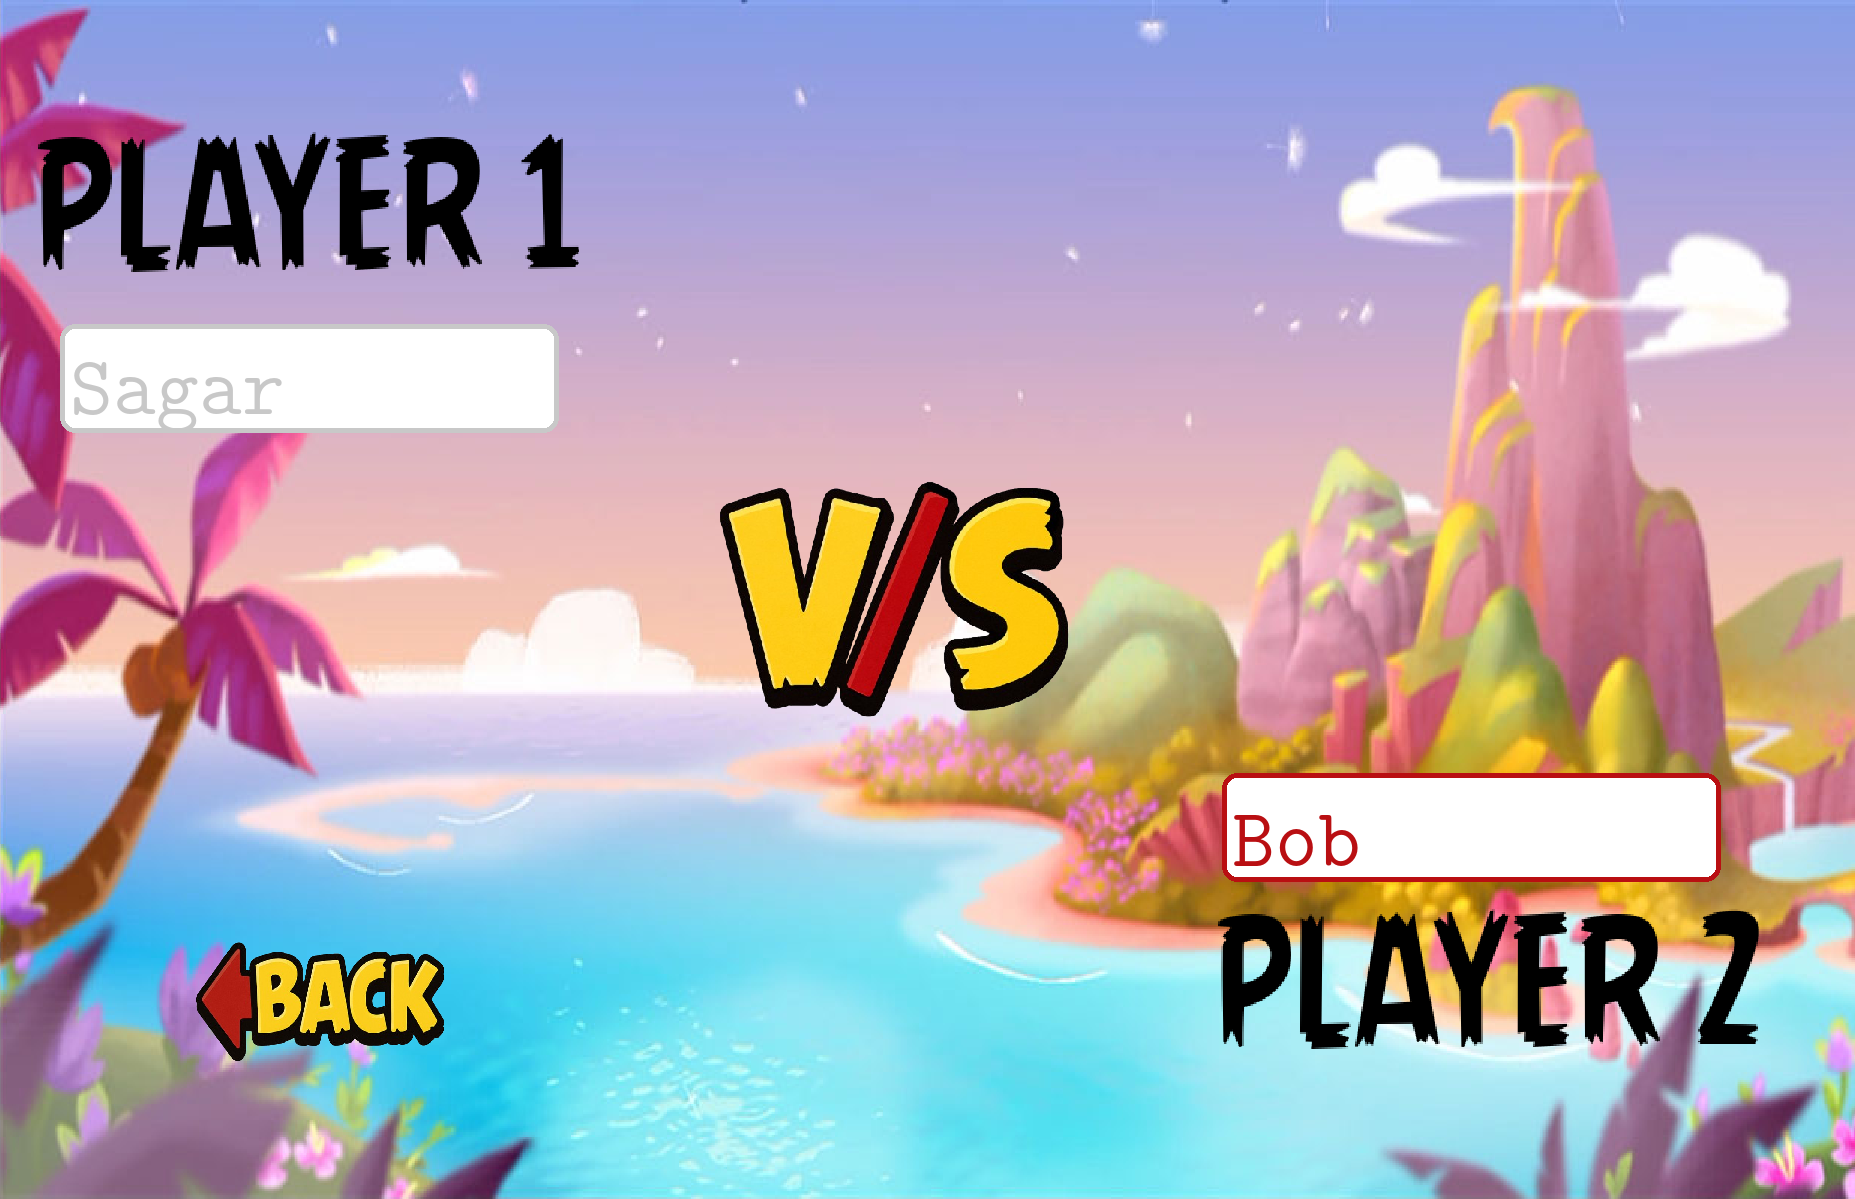
\includegraphics[width=0.5\textwidth]{Naming.png}
    \caption{Naming Interface}\label{fig:Name}
\end{figure}
\newpage
\subsubsection{Theme Selection}
This is where we select the theme for the actual gameplay[\ref{fig:Theme}]. Hovering over a theme enlarges it with a blue border and the corresponding theme music plays.
\begin{figure}[h]
    \centering
    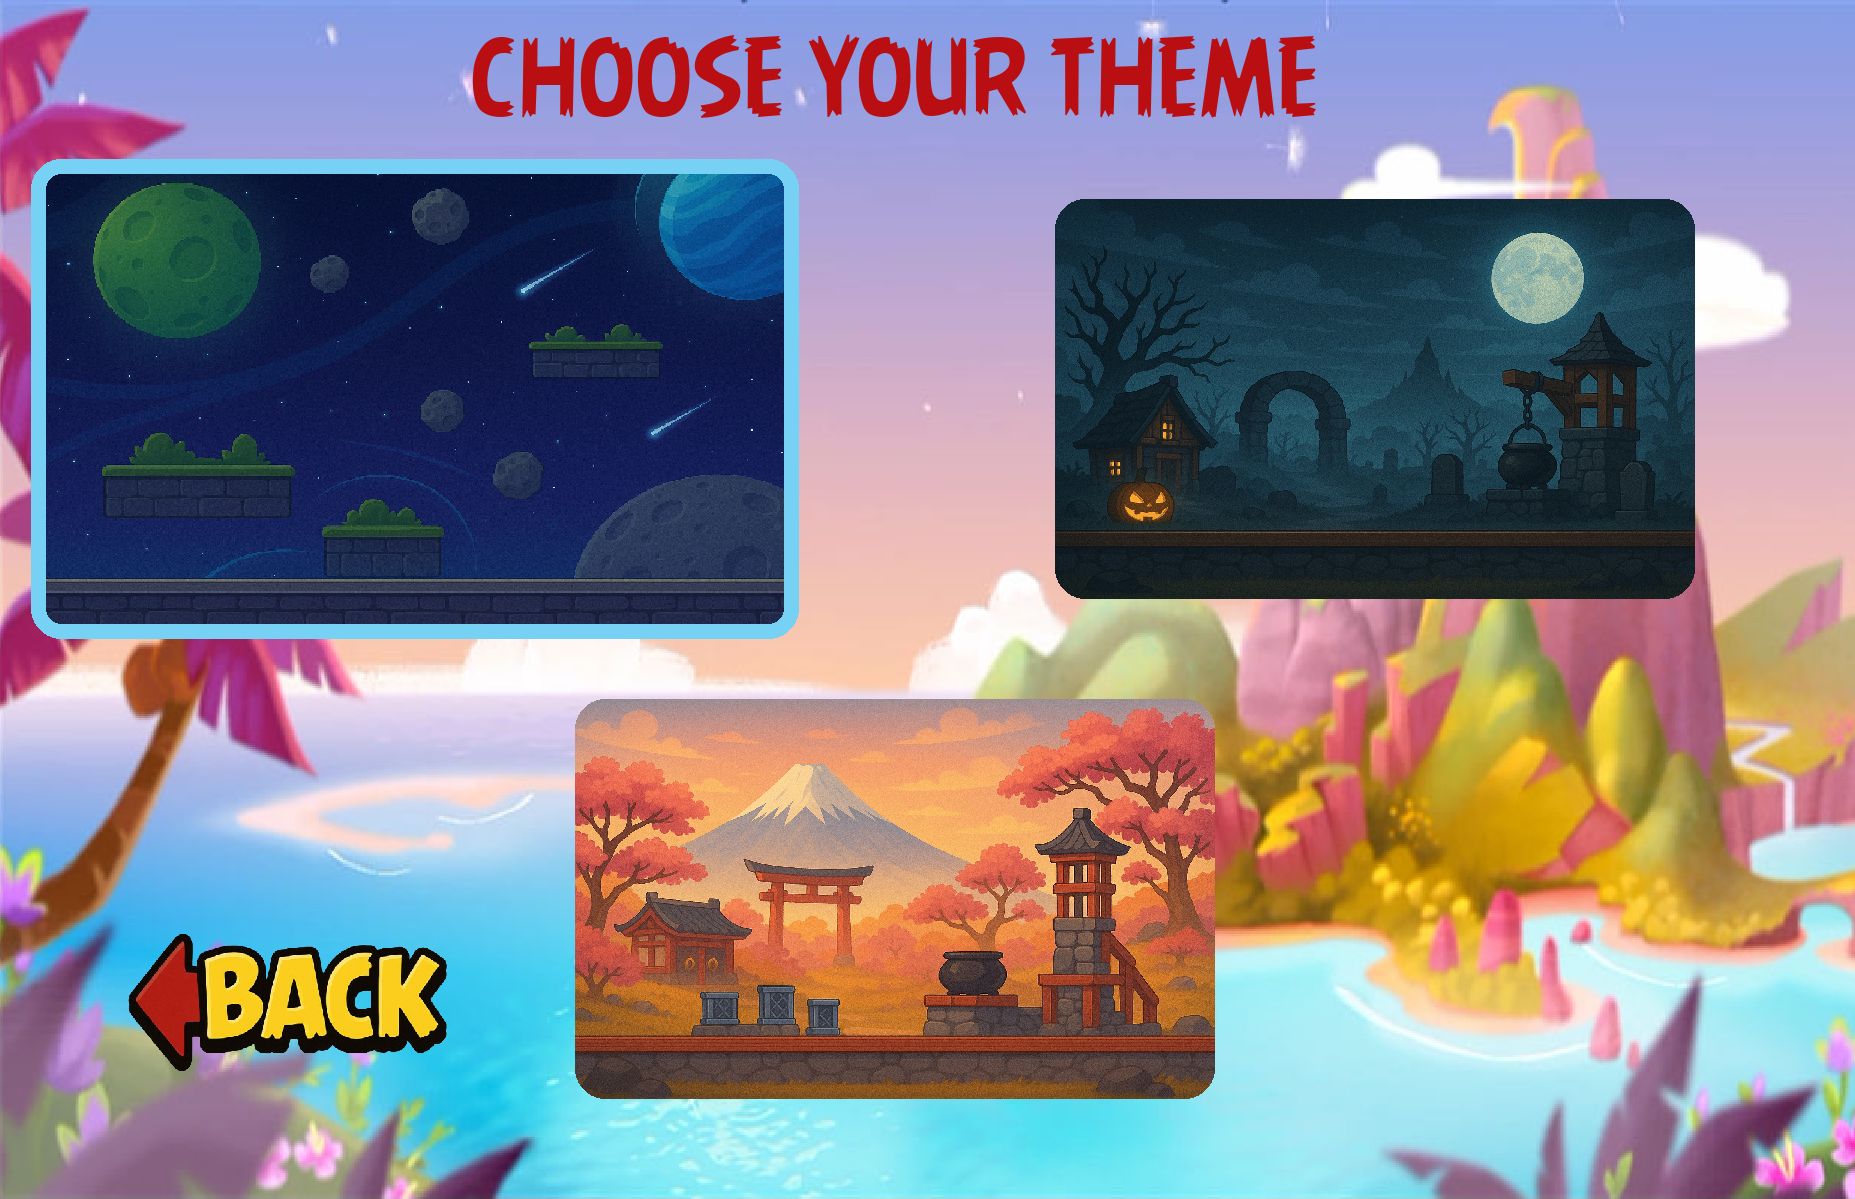
\includegraphics[width=0.5\textwidth]{Theme.png}
    \caption{Theme Select}\label{fig:Theme}
\end{figure}


\subsubsection{Bird Selection}
This is the unique bird selection menu. Each bird's information is displayed on mouse hover. Choosing it puts a tick over the bird.\\
The figure[\ref{fig:Select}] shows when \textbf{Red} is selected and mouse is hovering over \textbf{Bomb}.
\begin{figure}[h]
    \centering
    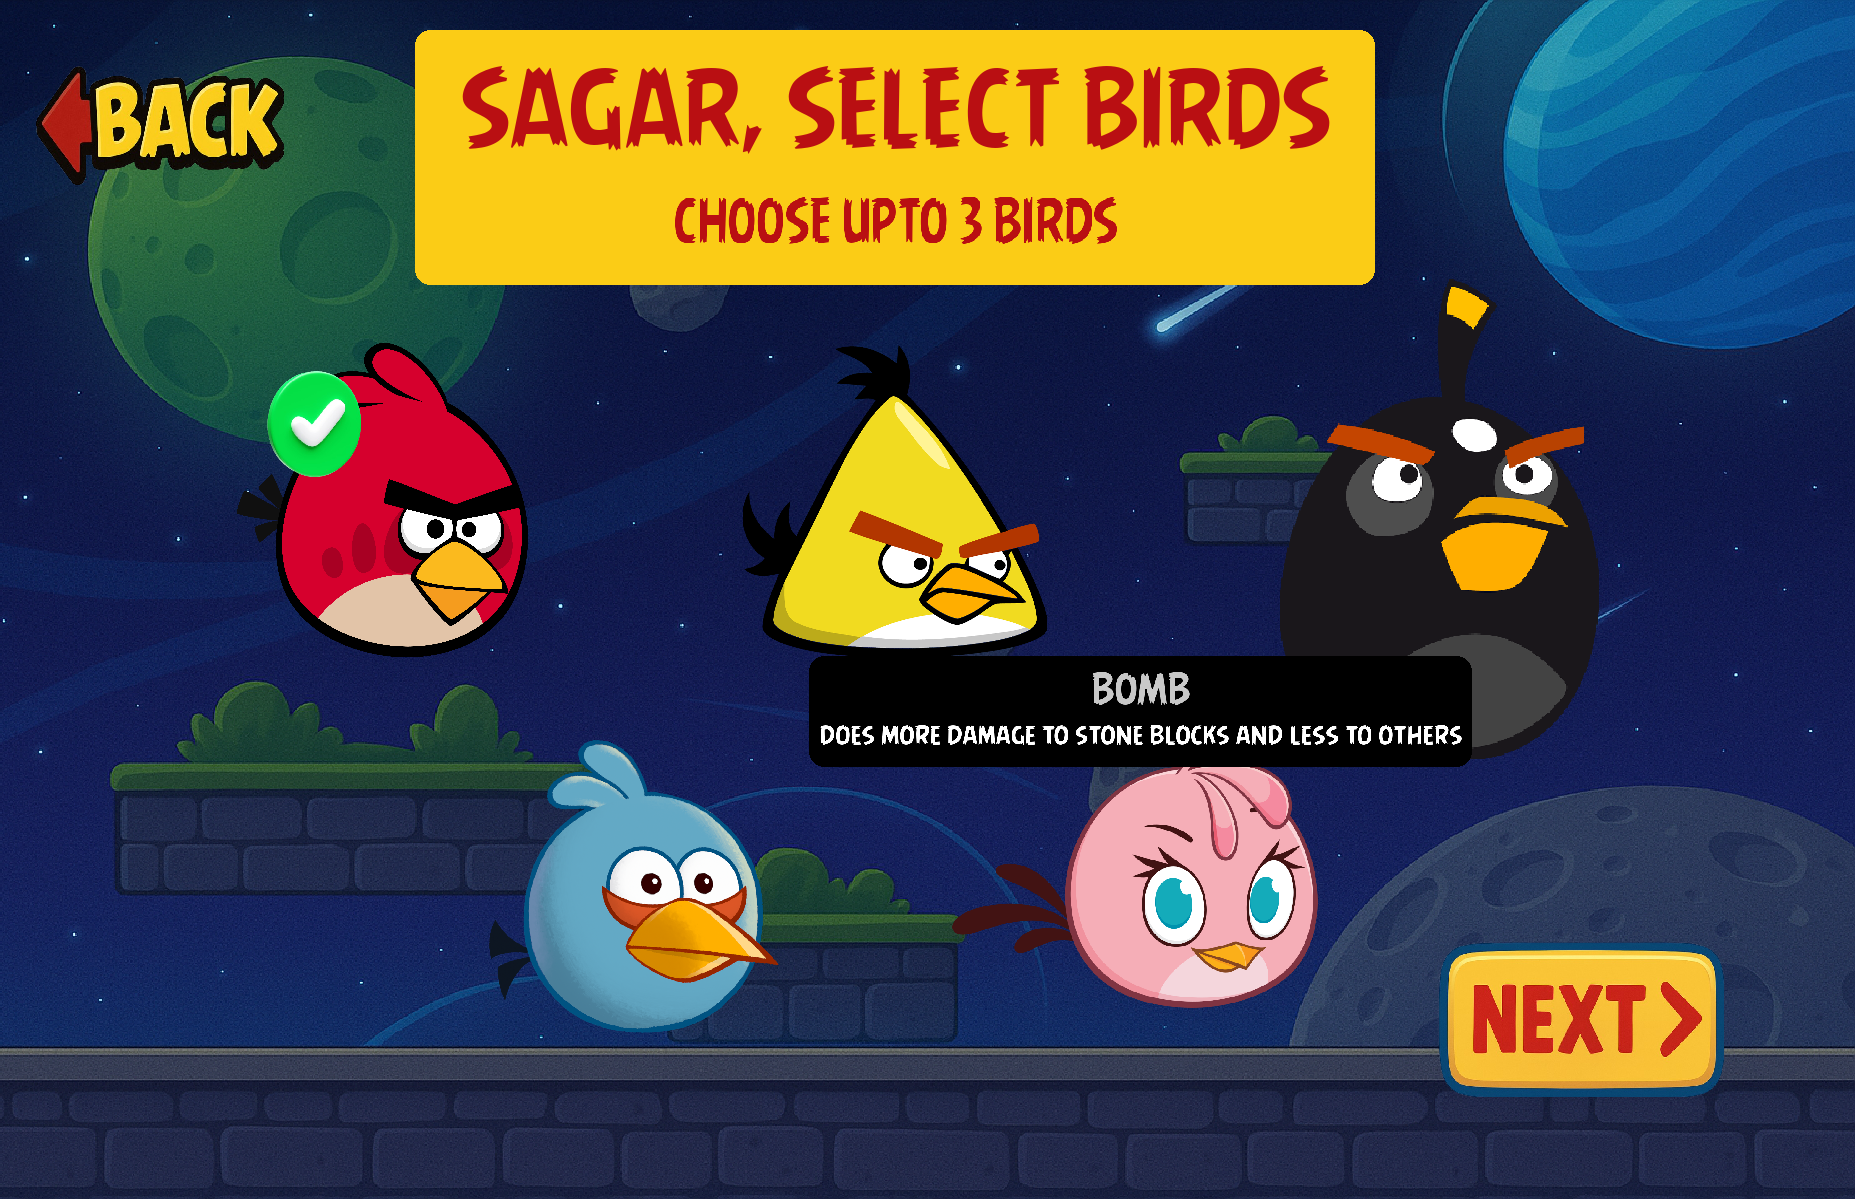
\includegraphics[width=0.5\textwidth]{Select.png}
    \caption{Bird Select}\label{fig:Select}
\end{figure}
\newpage
\subsubsection{PLAY}
This is the most comprehensive section of the game. This is where the actual gameplay happens.\\
\\This part starts of with a cool "FIGHT" animation[\ref{fig:Fight}]\\
\begin{figure}[h]
    \centering
    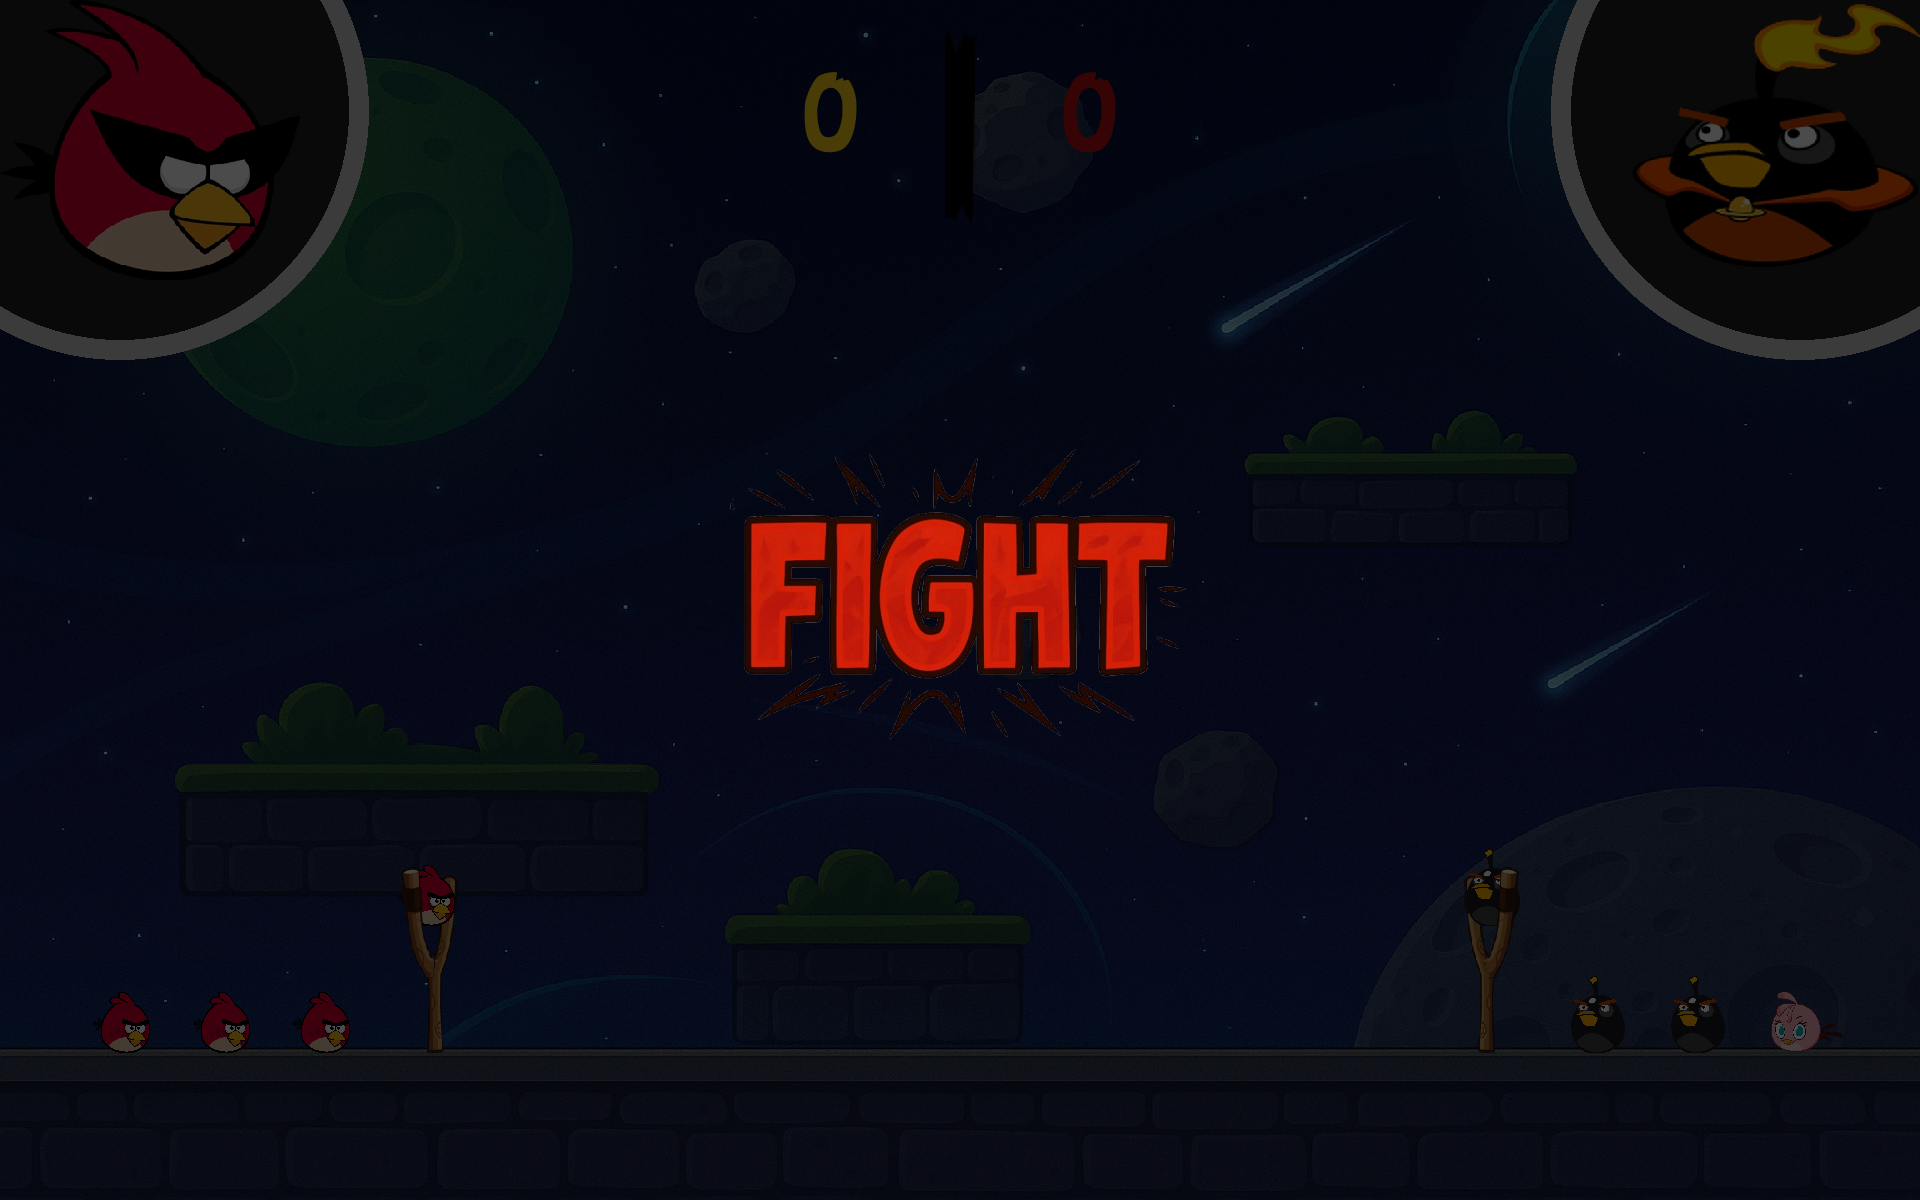
\includegraphics[width=0.5\textwidth]{Fight.png}
    \caption{FIGHT Animation}\label{fig:Fight}
\end{figure}

\begin{figure}[h]
    \centering
    \begin{subfigure}[b]{0.45\textwidth}
        \centering
        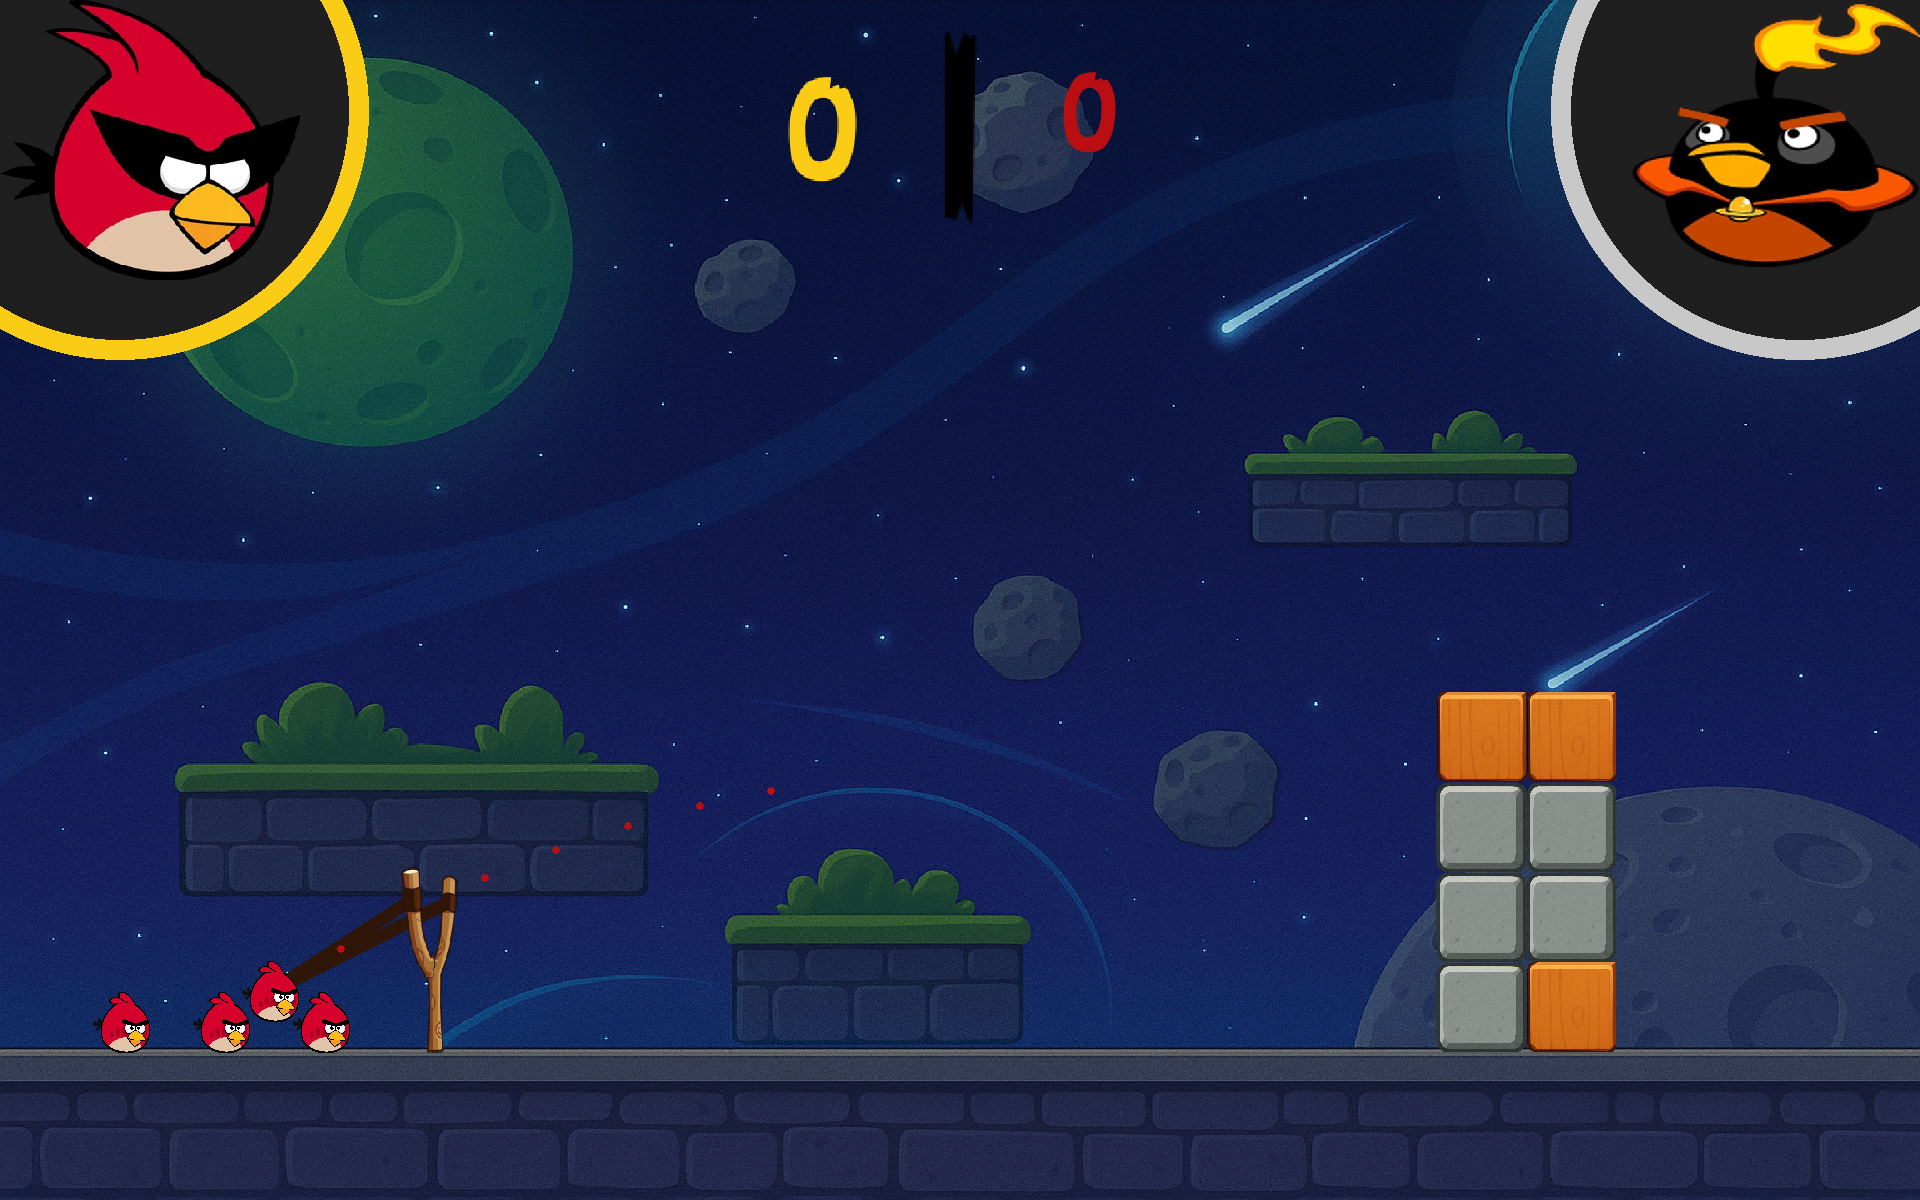
\includegraphics[width=\textwidth]{Player1.png}
        \caption{Player 1 Launching}\label{fig:P1}   
    \end{subfigure}
    \hspace{0.05\textwidth}
    \begin{subfigure}[b]{0.45\textwidth}
        \centering
        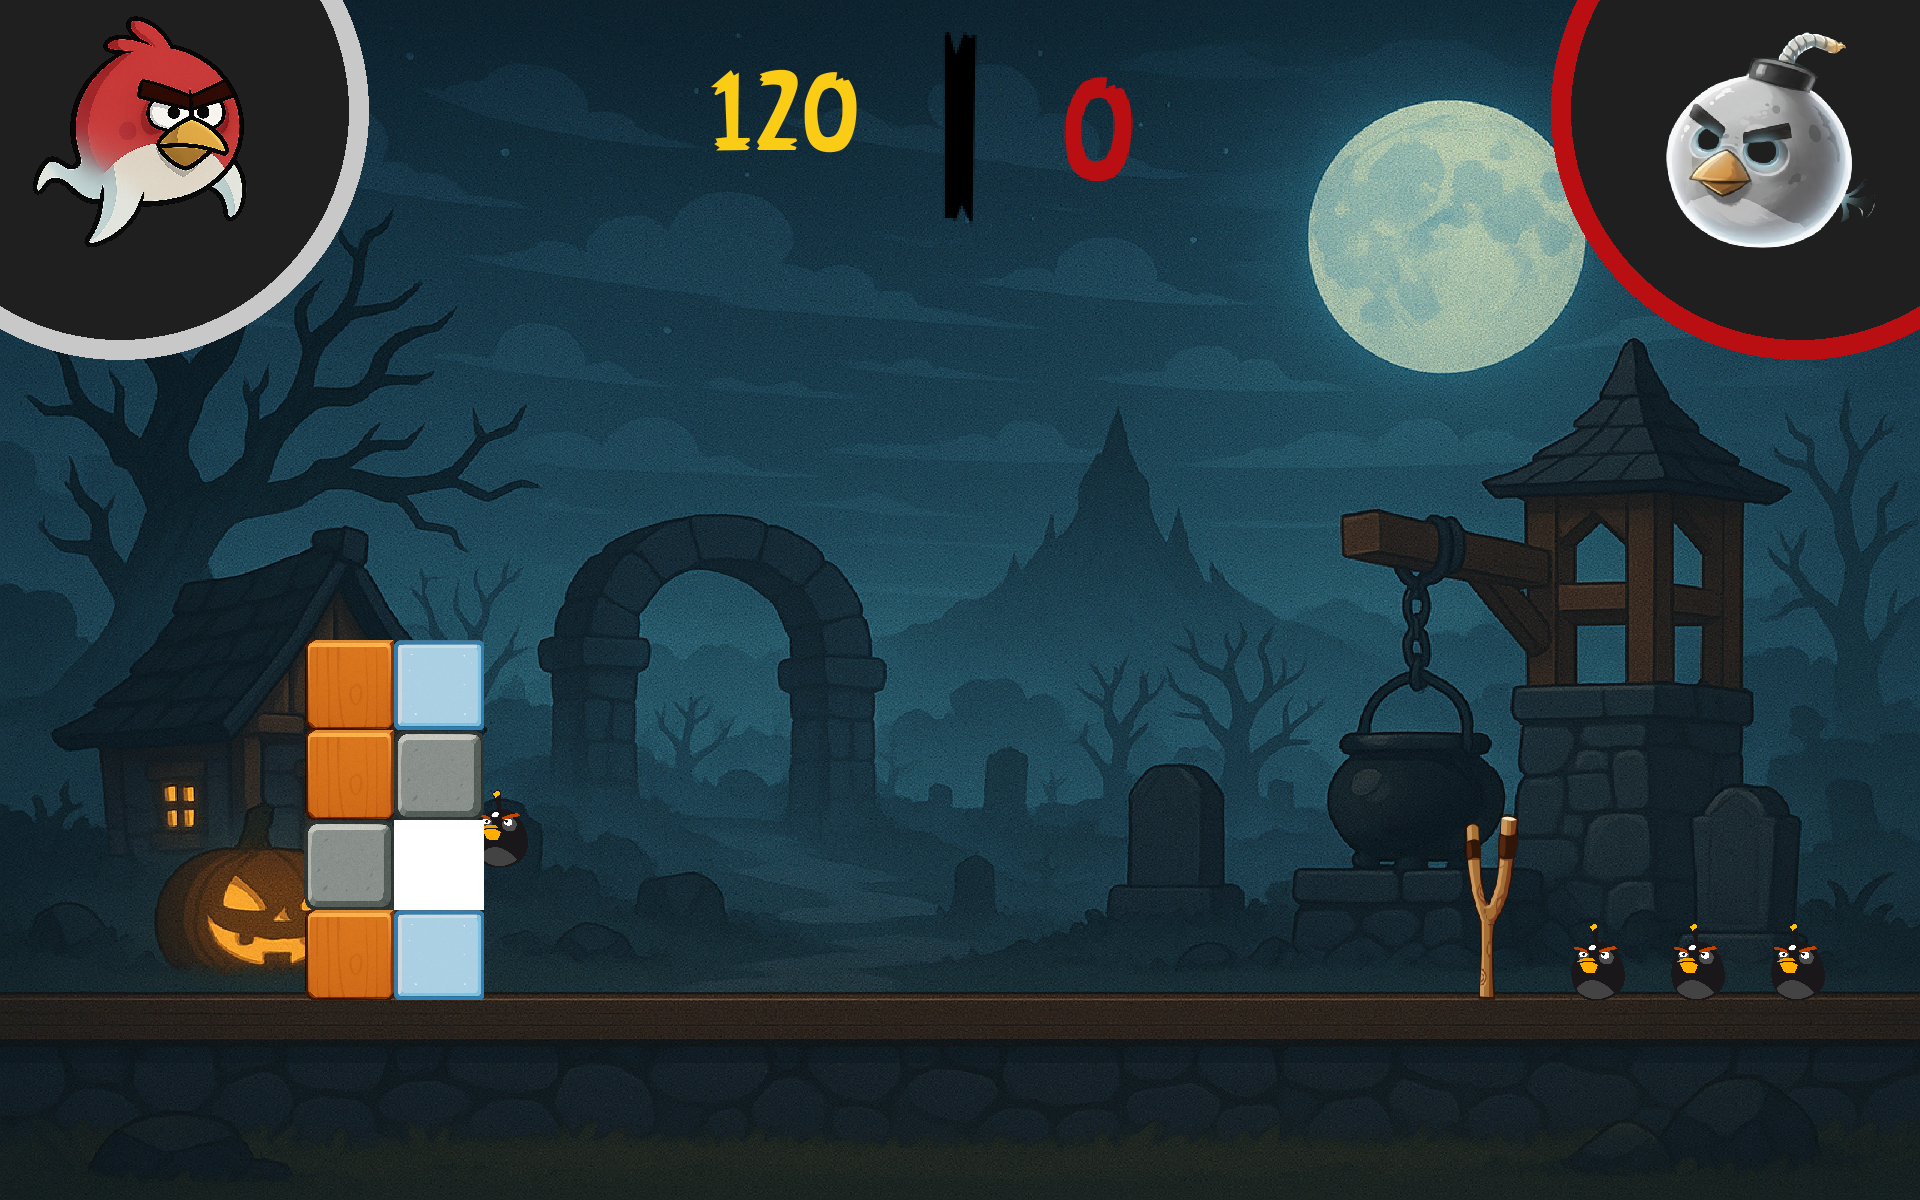
\includegraphics[width=\textwidth]{Player2.png}
        \caption{Player 2 Colliding}\label{fig:P2}
    \end{subfigure}
    \caption{Gameplay Interface}\label{fig:Playing}
\end{figure}

A cool feature in the gameplay screen[\ref{fig:Playing}] is the \textbf{Player Avatar} in the top right and left of the screen.\\
The latest bird for launching shows up as the avatar in different styles for different themes.\\
The Gameplay happens by a turn by turn basis, i.e., when Player 1 is launching, Player 2's slingshot and blocks are not visible, and vice versa.\\
\\In [\ref{fig:P1}], it is Player 1's turn. So, Player 1's avatar is highlighted and its score appears bigger than Player 2's. There are also tracking dots to help the players.\\
In [\ref{fig:P2}], the bird is colliding with block, the white highligh shows which block the bird collided with.
\\
\begin{figure}[h]
    \centering
    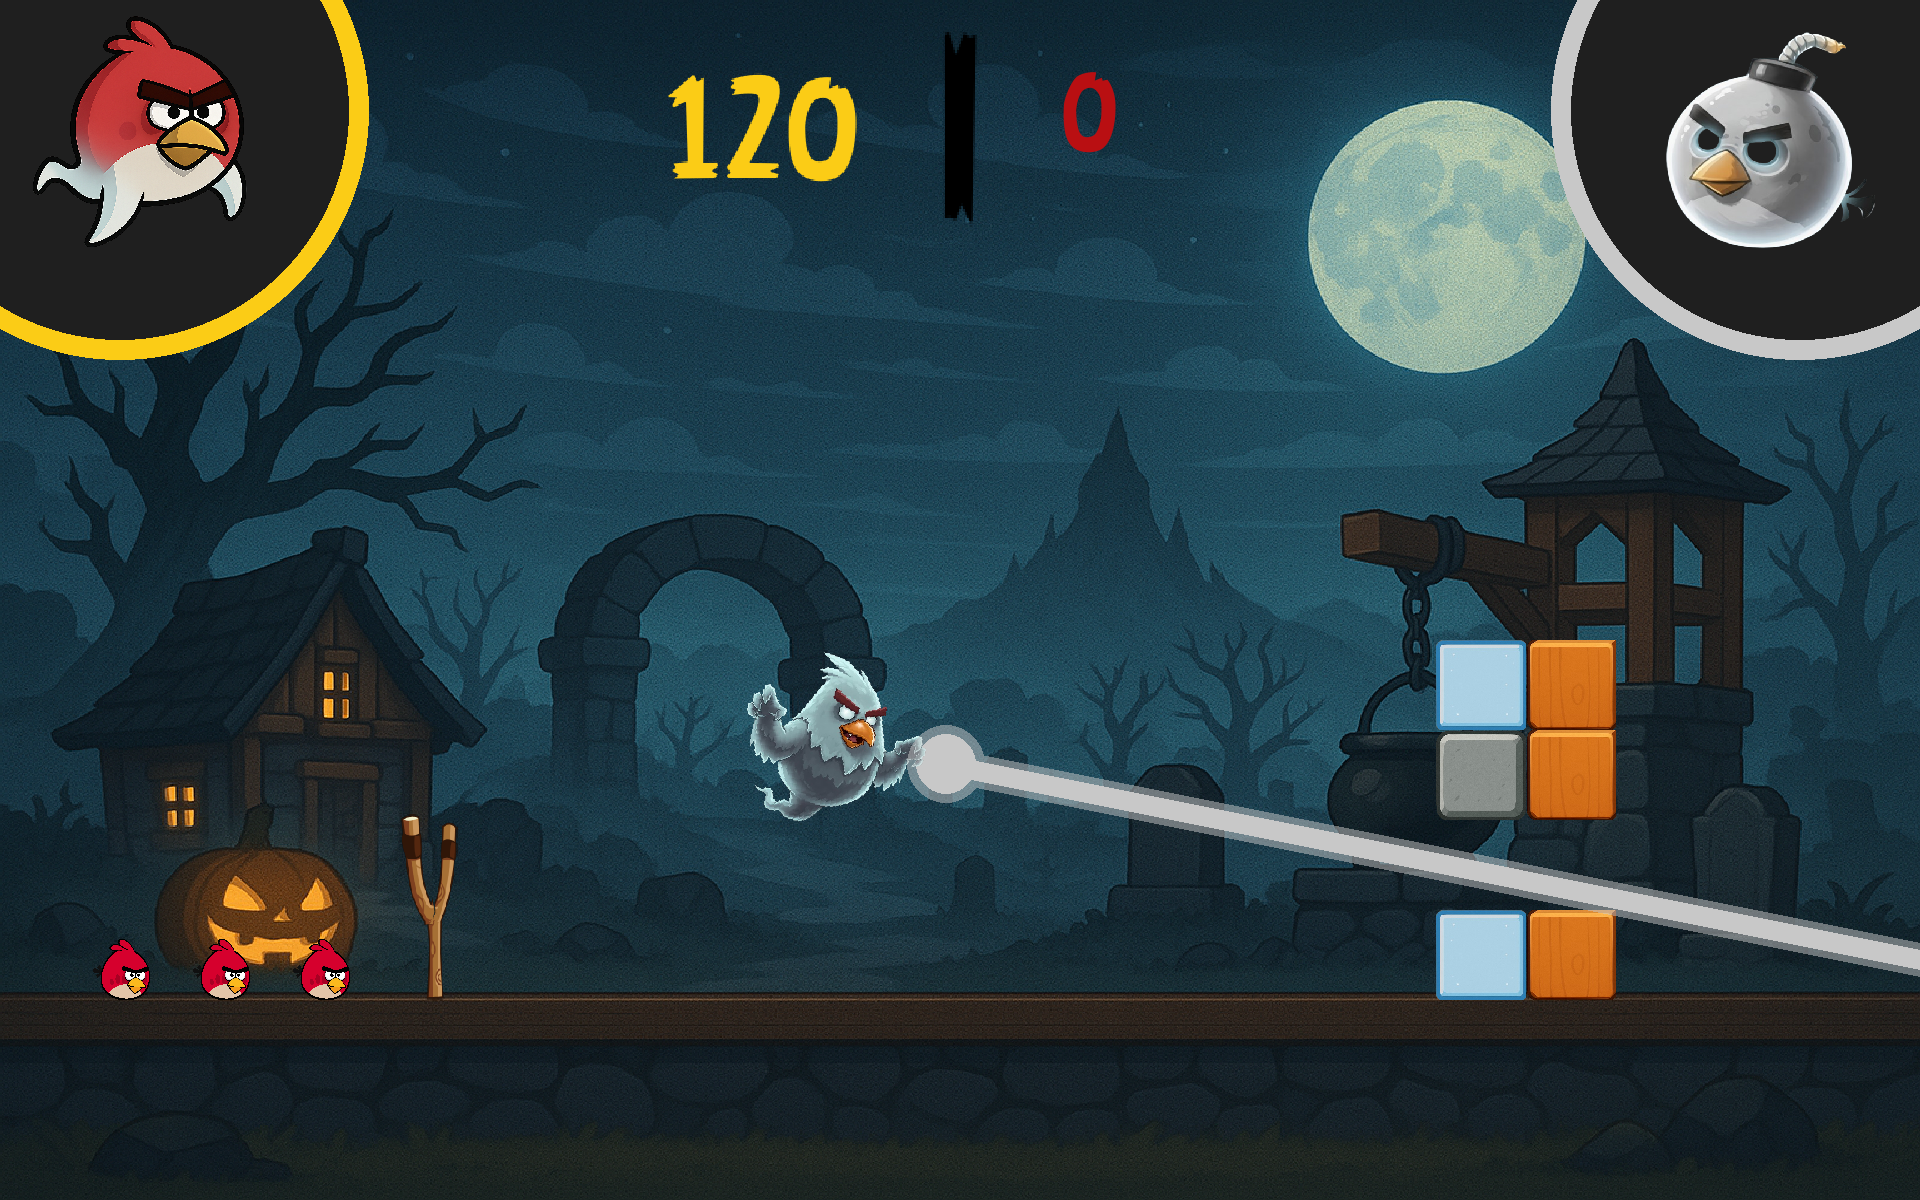
\includegraphics[width=0.5\textwidth]{Special.png}
    \caption{Special Ability Ghost Theme}\label{fig:Special}
\end{figure}

The figure [\ref{fig:Special}] shows us the special ability which can only be used once in a game by a player. It annihilates everything in its path.


\begin{figure}[h]
    \centering
    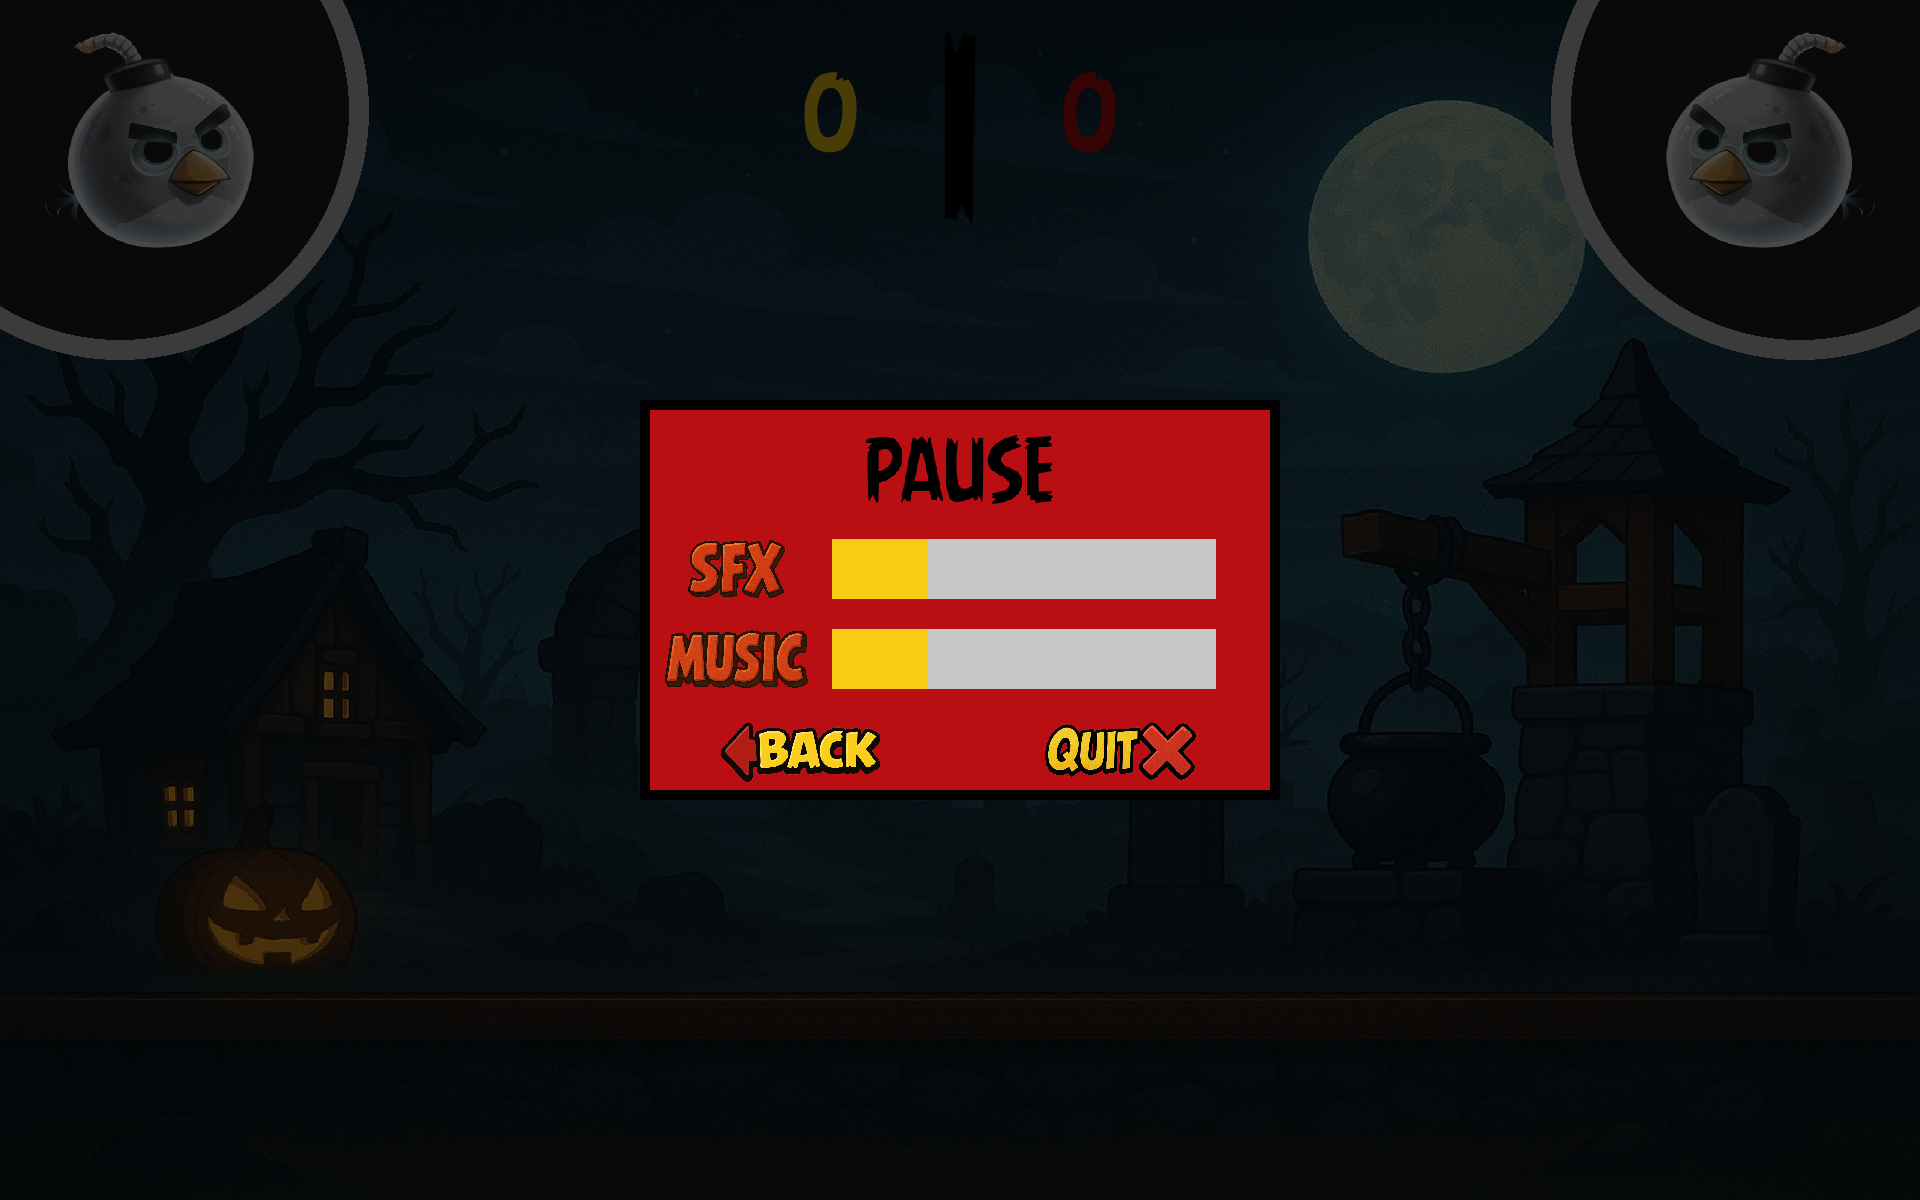
\includegraphics[width=0.5\textwidth]{Pause.png}
    \caption{Pause Menu}\label{fig:Pause}
\end{figure}
Figure [\ref{fig:Pause}] is the \textbf{Pause Menu} which pops up on clicking ESC key. It has volume controls and a \textbf{Quit} and \textbf{Back} button.


\newpage
\subsubsection{Winner}
This is the Winner screen[\ref{fig:Winner}]. It displays the winner of the game with \textbf{confetti} and even a \textbf{crown}.\\
It also has some great winner tunes to along with it.
\begin{figure}[h]
    \centering
    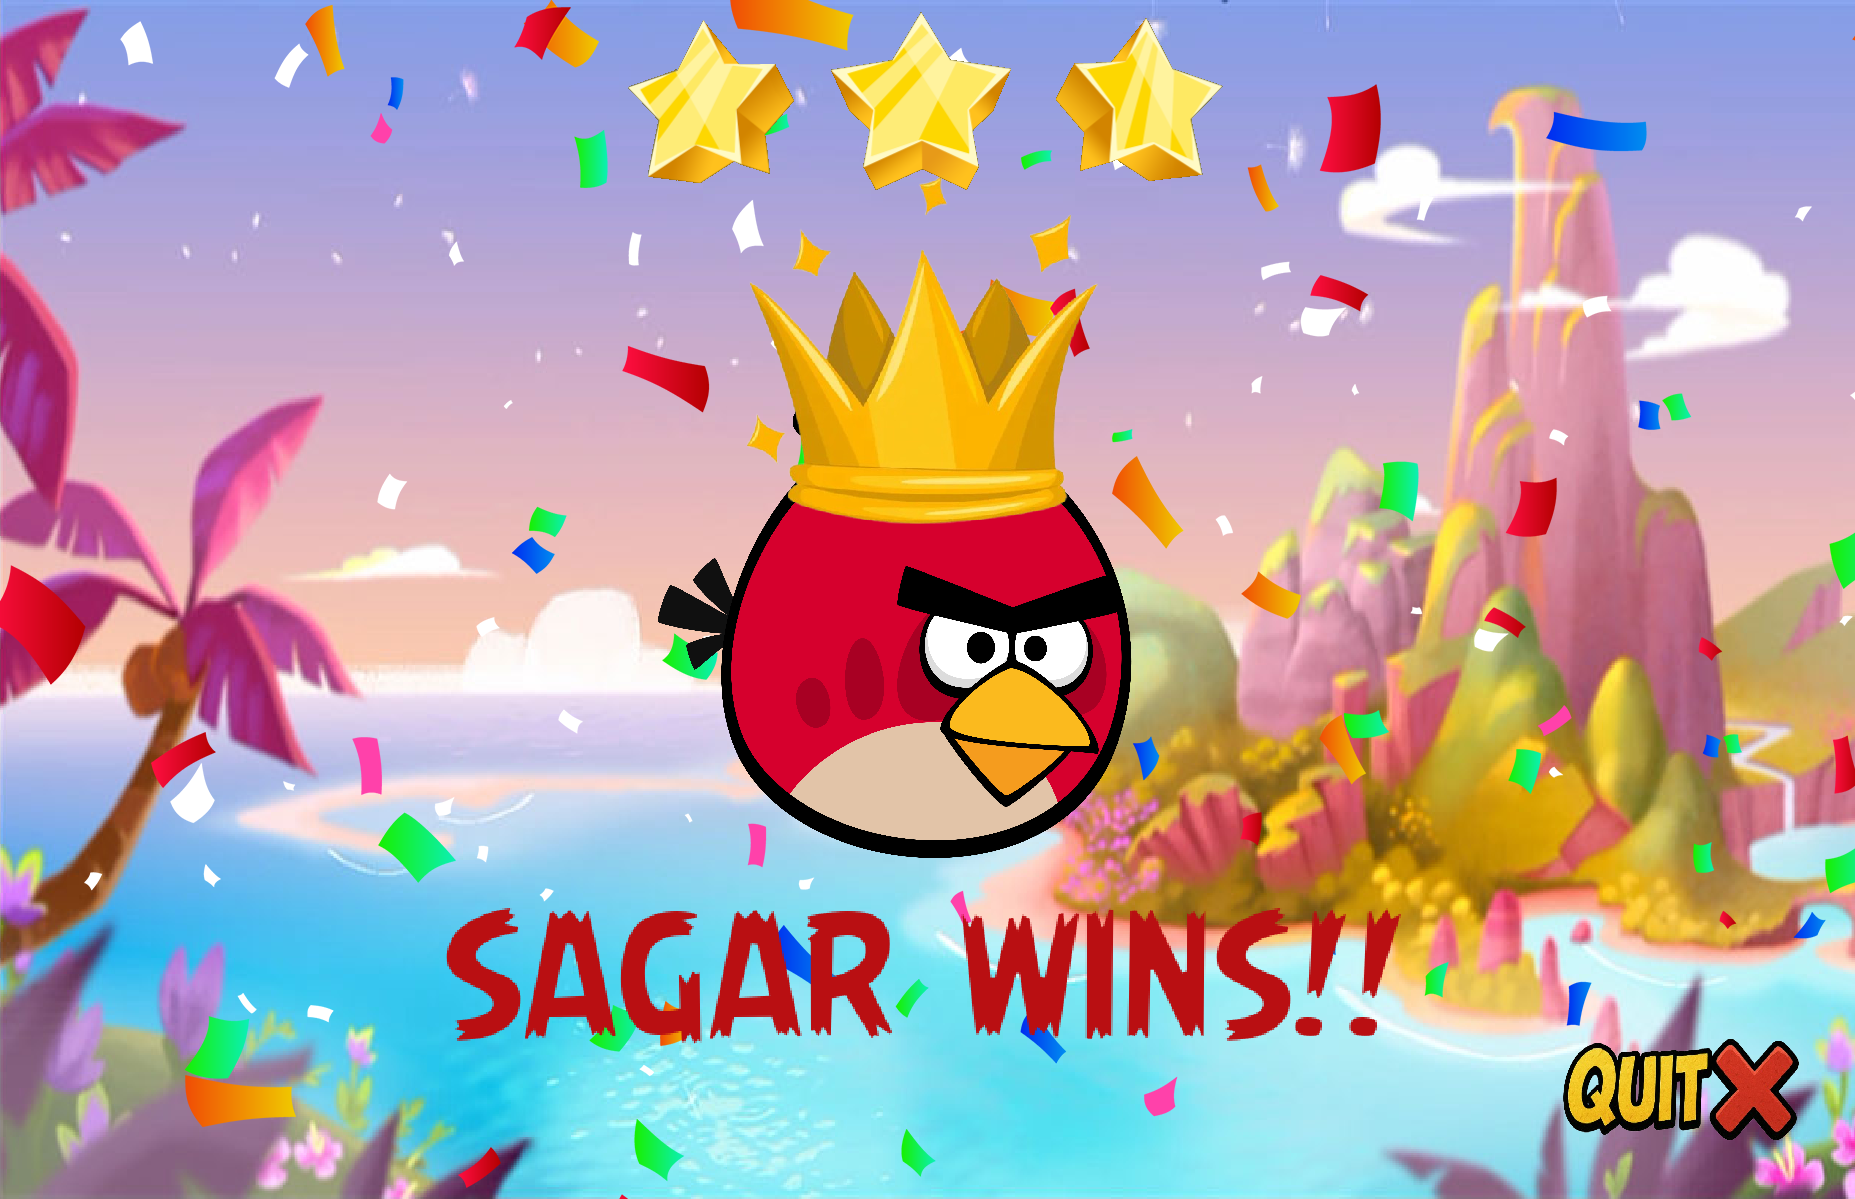
\includegraphics[width=0.5\textwidth]{Winner.png}
    \caption{Winner Screen}\label{fig:Winner}
\end{figure}

\section{Customization}
\begin{itemize}
    \item Animated Buttons -- size increases on hover
    \item Sound effects for button hover and clicks
    \item Menu options to change volume of background music and SFX independently
    \item Added a special ability, codename, \textbf{Mighty Eagle}
    \item Implementation of multiple themes -- themed soundtracks, birds and special ability.
    \item A comprehensive bird select menu with further customization with respect to block damage in the form of \textbf{Stella}
    \item Added \textbf{Player Avatars} indicating which bird they have currently equipped and whose turn it is.
    \item Added slingshot, bird launch and bird collision sound effects
    \item Implemented a cool scorecard animation
    \item Custom font
\end{itemize}

\begin{thebibliography}{9}
    \bibitem{pygameDoc}
    Pygame Official Documentation\
    \url{https://www.pygame.org/docs/}
\end{thebibliography}

\end{document}